\chapter{INTRODUCTION}


\section{Global Renewable Energy Status}
Renewable energy is still one of the hottest topics in the power area. The share of the renewable energy systems has been reached significant levels. At the end of 2016, the renewable power capacity has reached 2011 GW throughout the world including hydropower plants.\cite{InternationalRenewableEnergyAgency2017}  The renewable capacity for the leading countries is given in the Figure \ref{renewablecap}.Almost half of this capacity belongs to four leading countries namely; China, USA, Brazil and Germany.
\begin{figure}[h!]
	\centering
	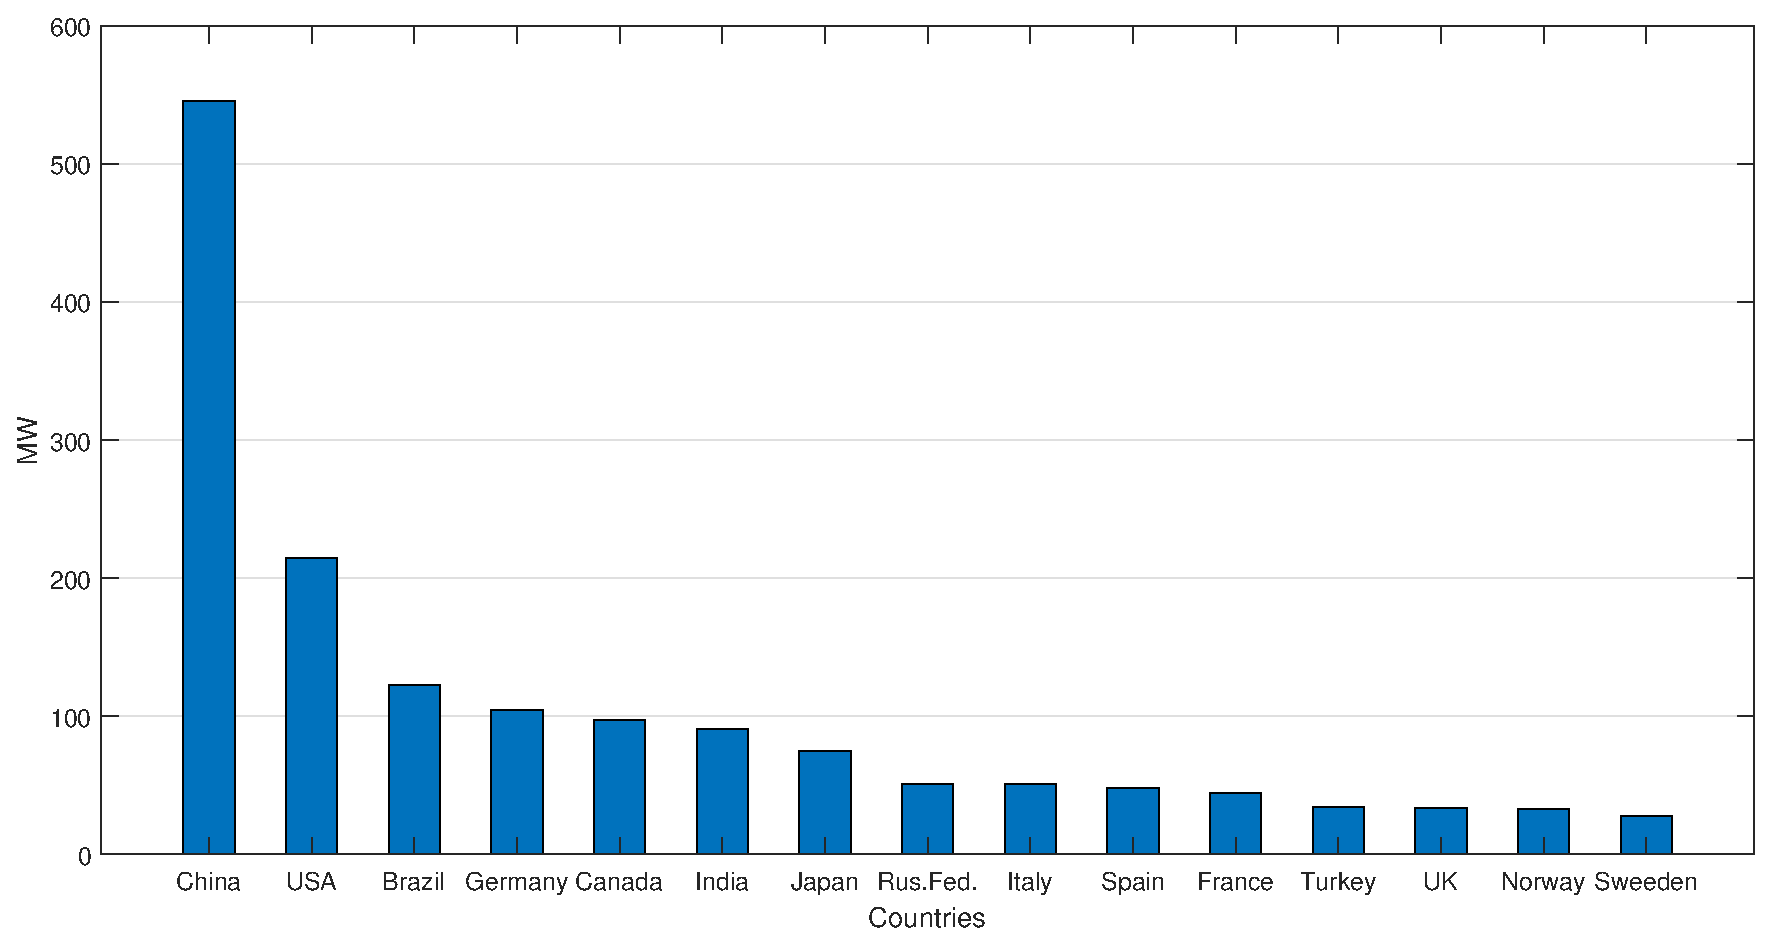
\includegraphics[scale=0.47]{renewablecapacity.eps}
	\caption{Installed Renewable Energy Capacity of Leading Countries in 2016\cite{InternationalRenewableEnergyAgency2017}}
	\label{renewablecap}
\end{figure}
Figure \ref{renewablepro} shows the energy production from renewable energy systems. It is clear that China, USA and Brazil produces highest amount of energy from renewable since they already have the highest installed capacity. However, India and Canada produces more energy than Germany even though Germany has more installed capacity. This result is due to the fact that renewable energy system production is dependent on parameters such as solar radiation and wind speed depending on the renewable source.
\begin{figure}[h!]
	\centering
	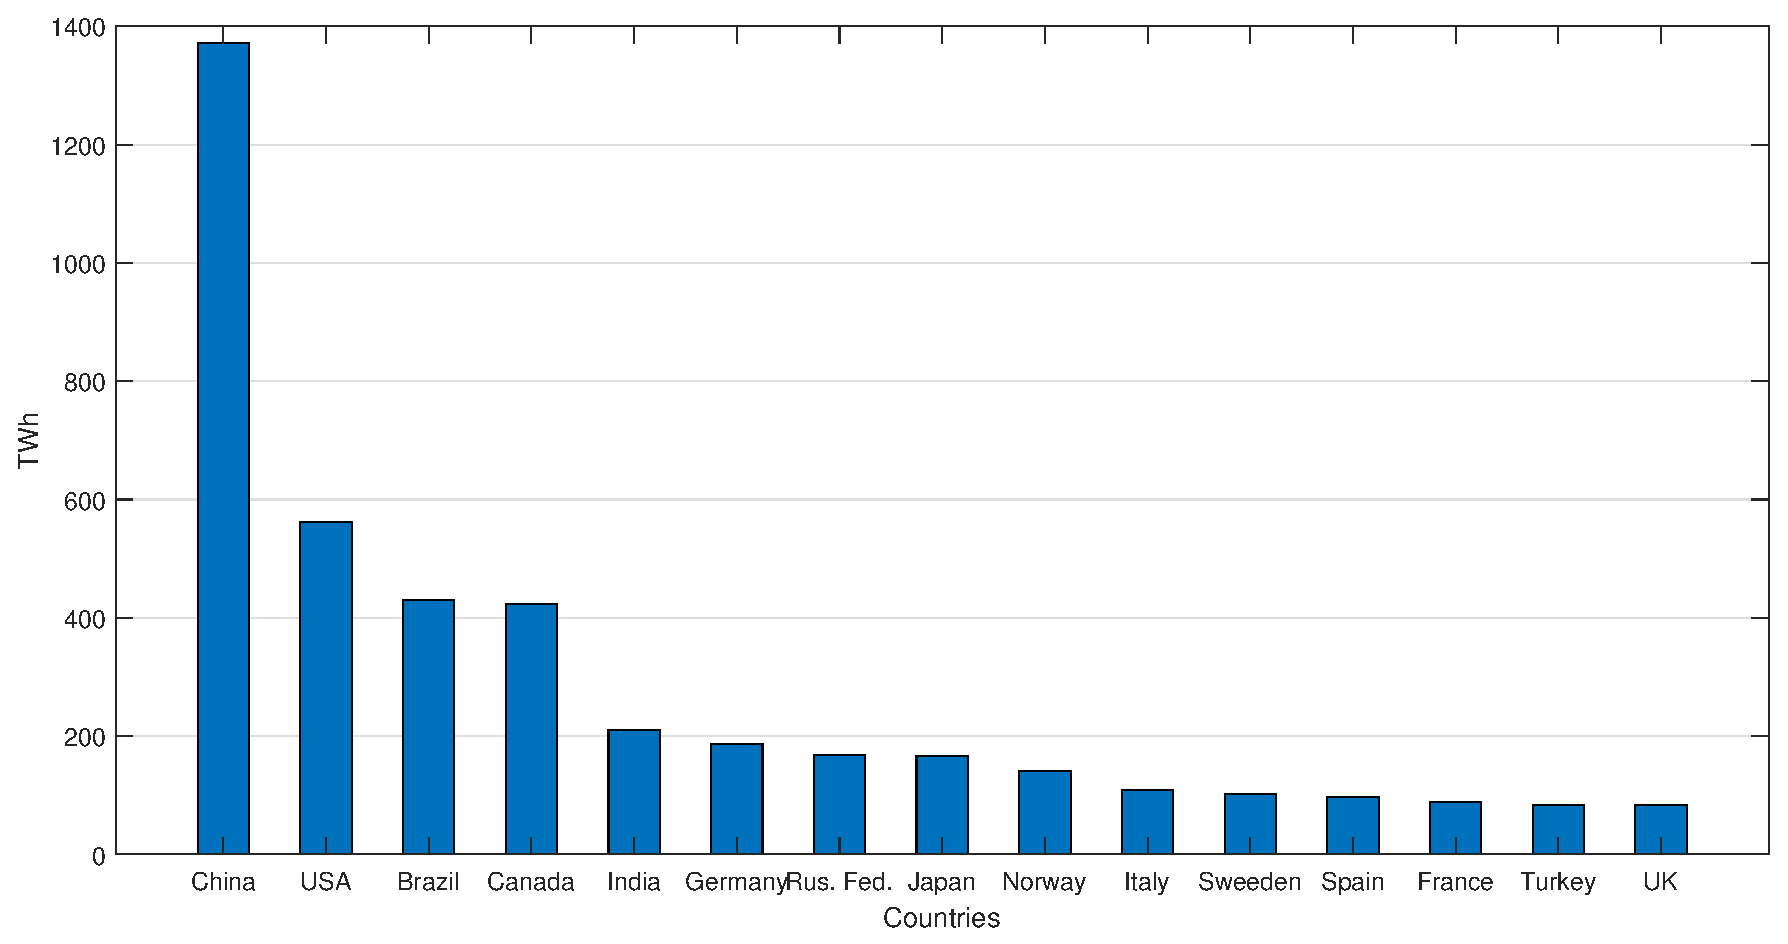
\includegraphics[scale=0.47]{renewableproduction.eps}
	\caption{Renewable Energy Production of Leading Countries in 2016 \cite{InternationalRenewableEnergyAgency2017}}
	\label{renewablepro}
\end{figure}


\section{EU 2020 Goals}
In 2008, 20 20 by 2020-Europe's Climate Change Opportunity report has been released by EU Commission and two key targets are set for 2020 \cite{EuropeanCommission2008}: 
\begin{itemize}  
	\item At least 20 \% reduction in greenhouse gases (GHG) by 2020
	\item Achieving 20\% renewable energy share in energy consumption of EU by 2020
\end{itemize}
The Renewable Energy Directive is published in 23 April 2009. This directive has set national binding targets for EU countries in order to accomplish the 20\% renewable energy target for EU and 10 \% target for the renewable energy usage in the transport. \cite{EuropeanParliament2009} As a result, each EU country has been determined their national action plans. In order to achieve the 20 \% target, each member state determine their own targets ranging from 10\% in Malta to 49\% in Sweeden. 
According to the latest release by Eurostat, renewable share of the EU in energy consumption has reached 17 \% in 2016 \cite{States2016}. Moreover, eleven of EU member states has already achieved their 2020 targets. Renewable shares of EU members are shown in Figure \ref{EUtargets}.
\begin{figure}[h!]
	\centering
	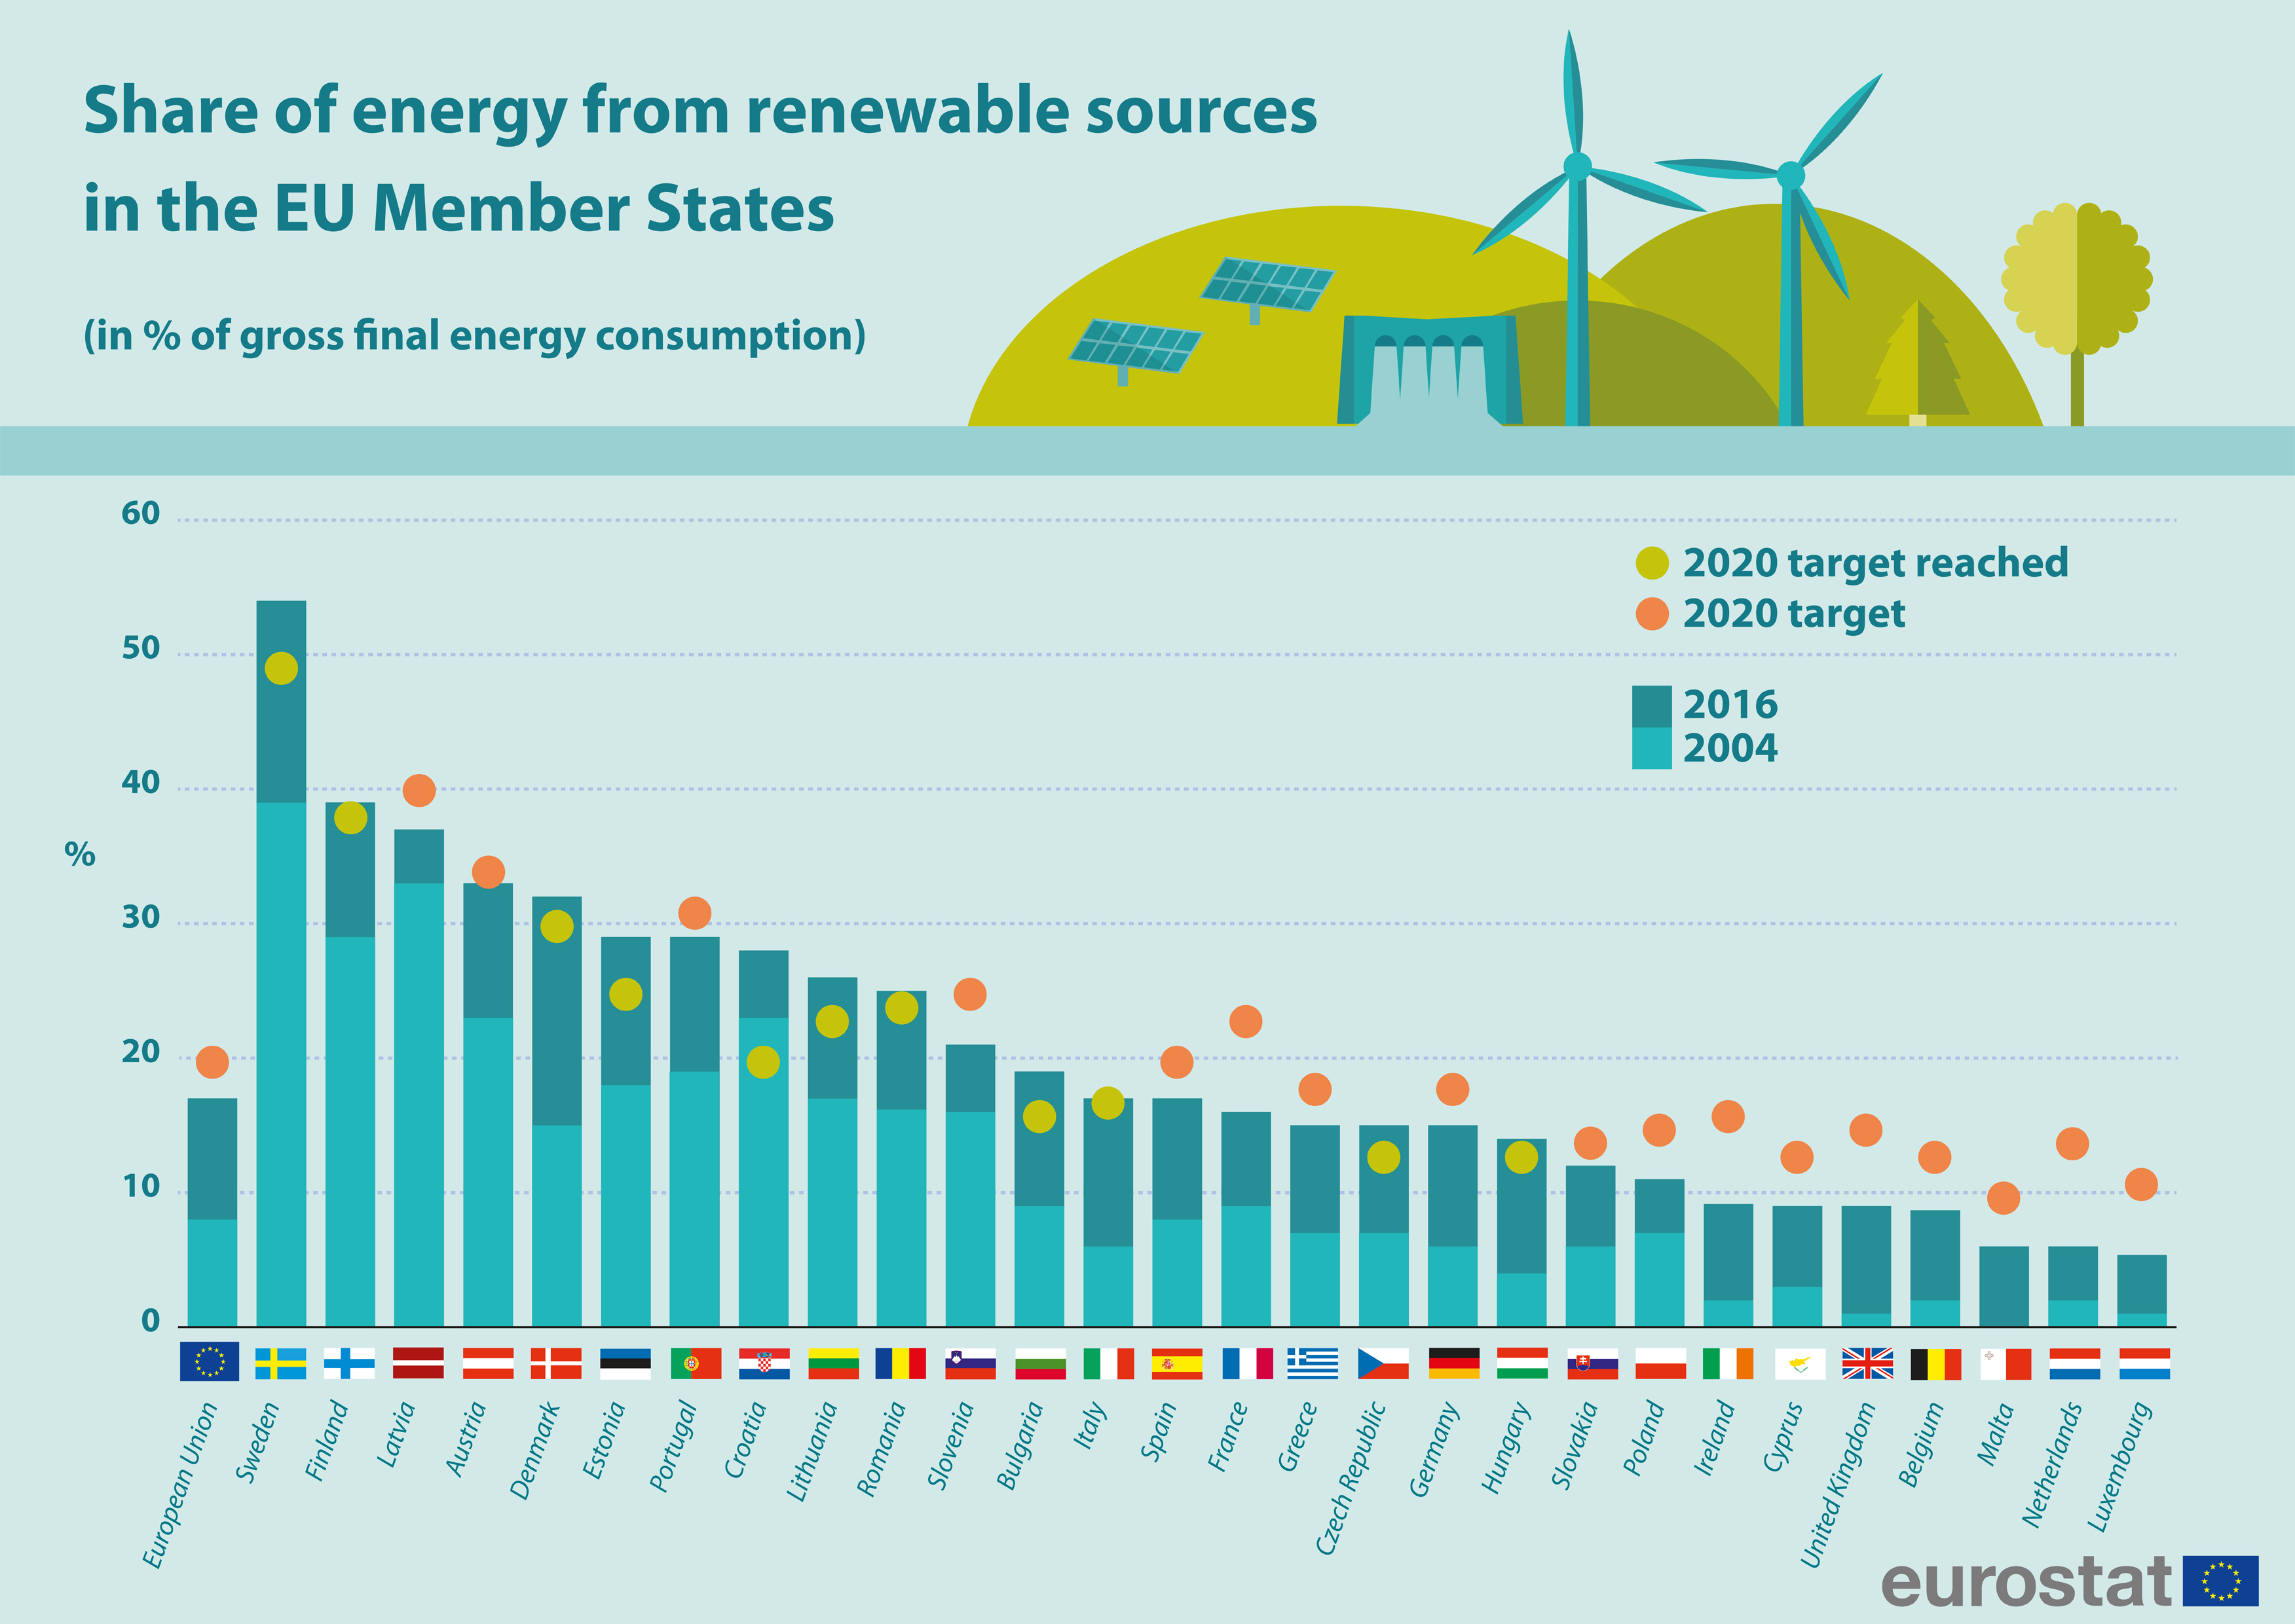
\includegraphics[scale=0.12]{Figure_1-Share_of_energy_from_renewable_sources_2004-2016.png}
	\caption{Renewable Targets of EU Member States\cite{States2016}}
	\label{EUtargets}
\end{figure}


\section{Wind Energy Status}
Wind power has the highest share in the renewable energy except for hydropower. The wind power capacity at the end of 2016 has reached 467 GW worldwide. The wind power capacity of the leading countries are given in the Figure \ref{windcap}. China and USA have also the highest installed capacities in the wind power. Moreover, it should also be noted that the share of the wind power in the total installed capacity is more important that total wind power capacity
\begin{figure}[h!]
	\centering
	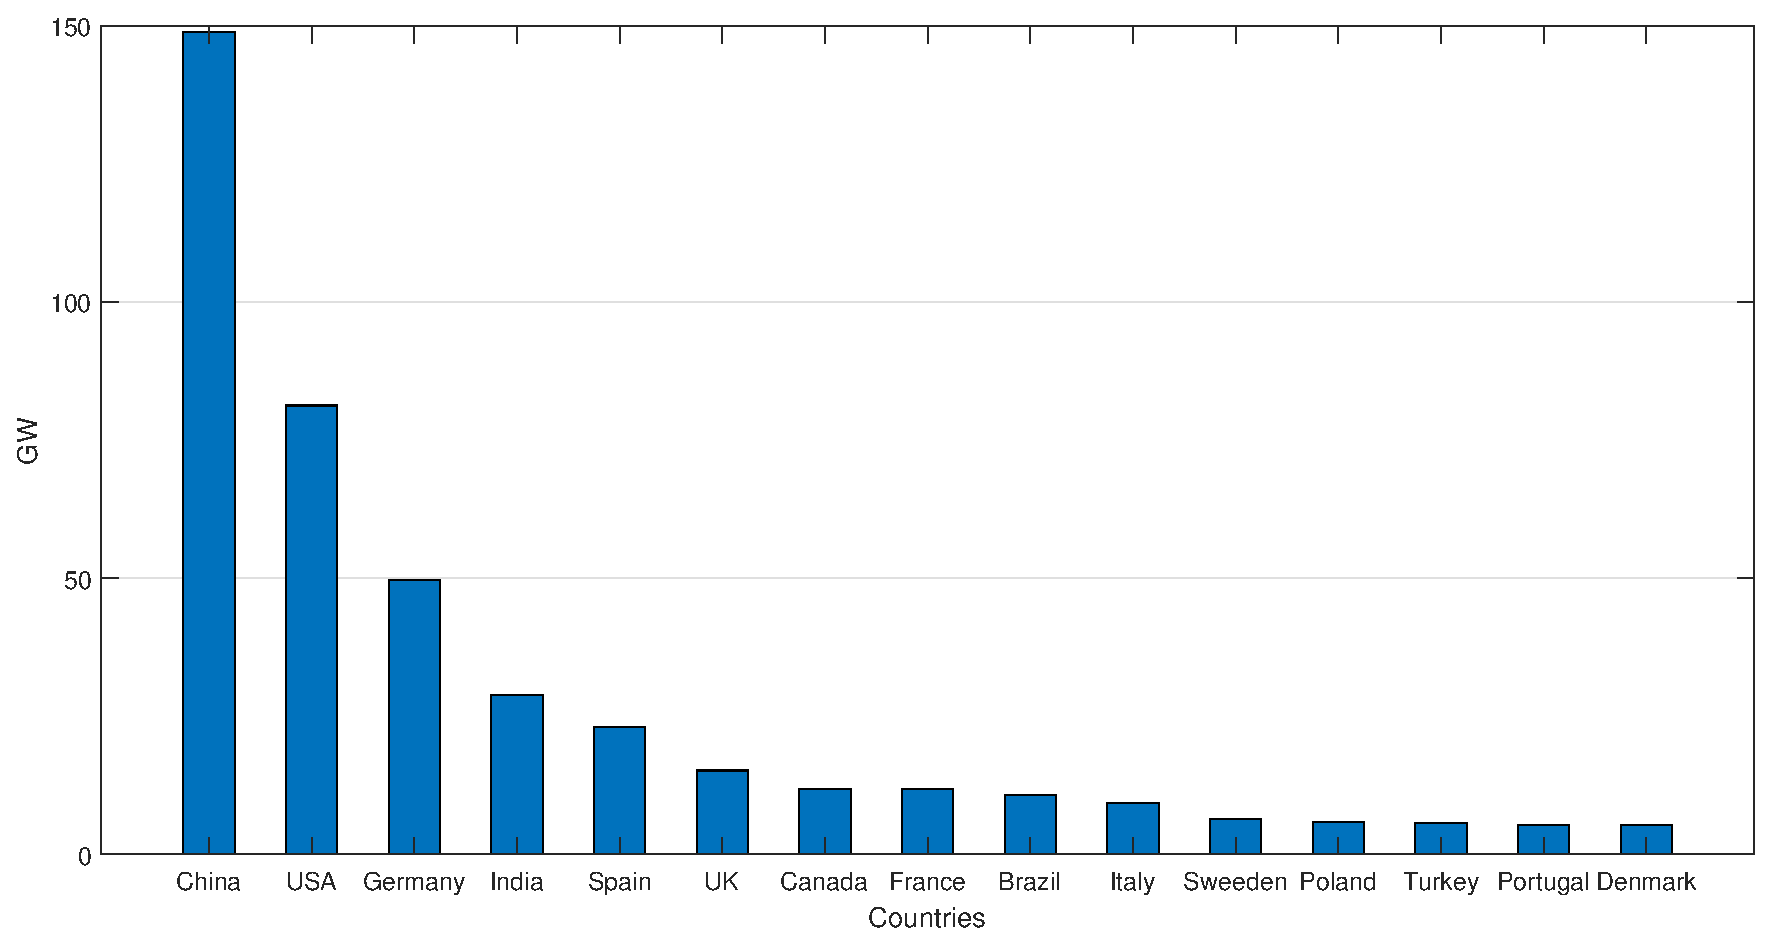
\includegraphics[scale=0.47]{windcapacity.eps}
	\caption{Wind Power Capacity of Leading Countries in 2016\cite{InternationalRenewableEnergyAgency2017}}
	\label{windcap}
\end{figure}
The energy production from wind energy is shown in the Figure \ref{windpro}. Even though China has the highest wind power capacity,  USA generates more energy from wind than any other country. 
\begin{figure}[h!]
	\centering
	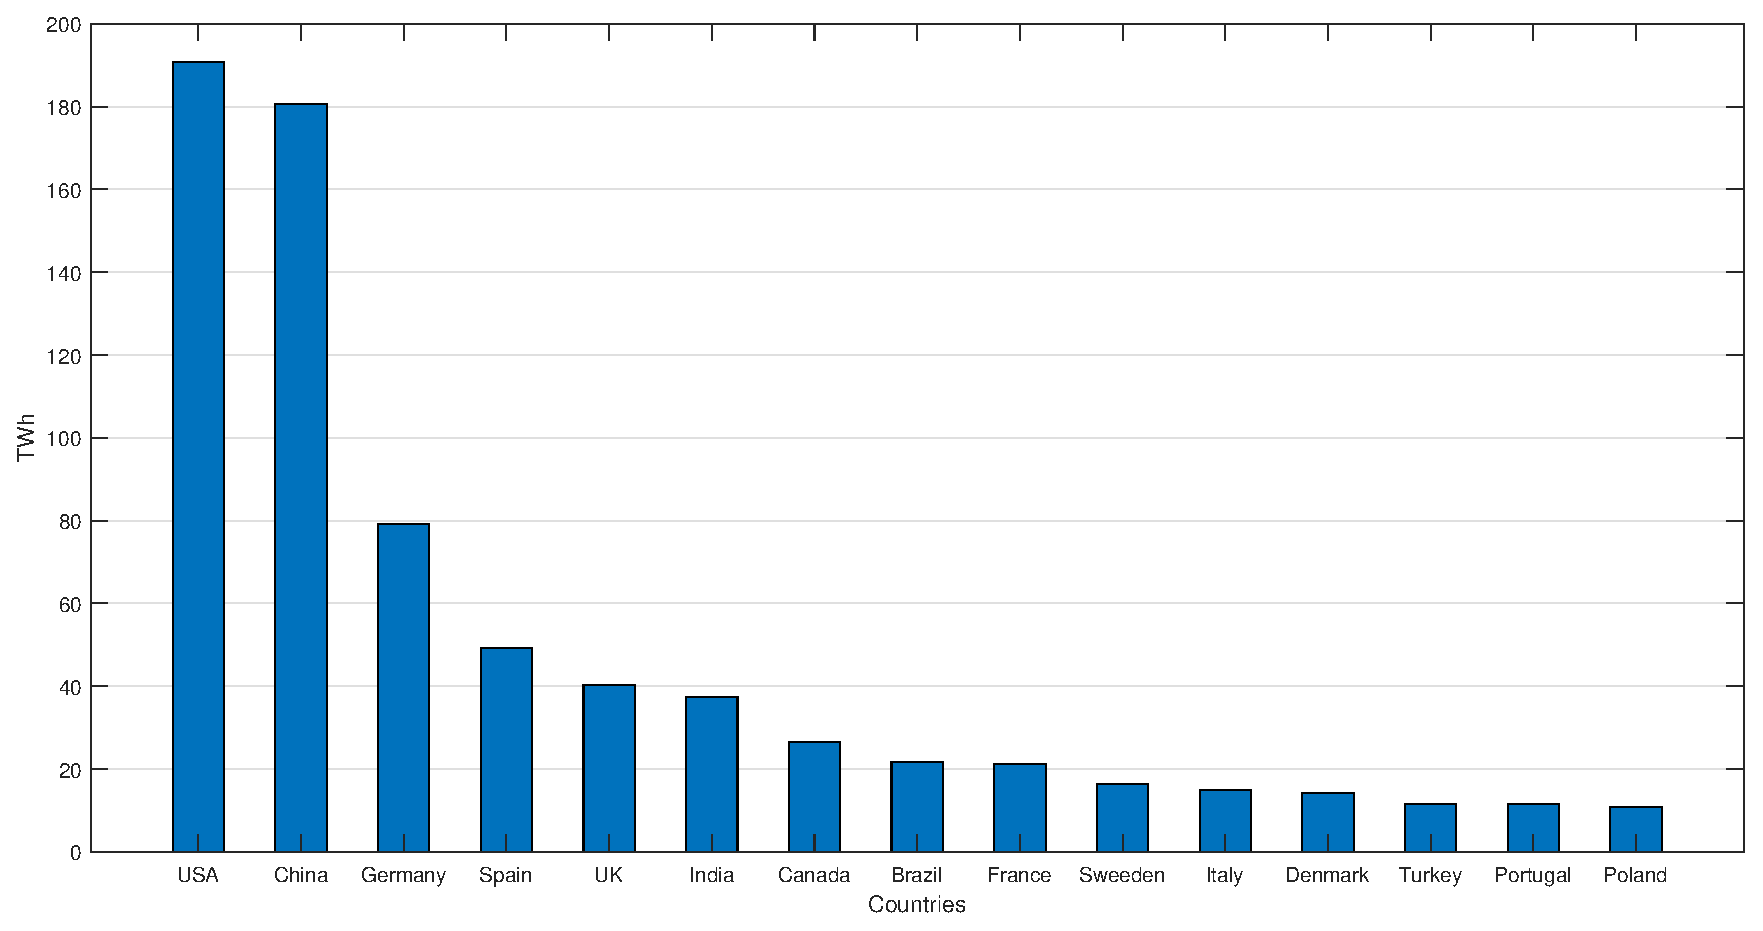
\includegraphics[scale=0.47]{windproduction.eps}
	\caption{Wind Power Production of Leading Countries in 2016\cite{InternationalRenewableEnergyAgency2017}}
	\label{windpro}
\end{figure}


\section{Global Renewable Energy Future}
The share of renewable energy is increasing each passing day. Today, reports arguing the possibility of even 100\% renewable energy region by region is published\cite{REN212017d}. The renewable energy reports estimate the share of renewable energy in the total energy consumption for 2030 and 2050. Figure \ref{EU2030} shows the EU renewable energy share for 2030. Moreover, the report published by IRENA (International Renewable Energy Agency) estimates the share of renewable energy in EU as 24\% by 2030 which is below proposed target of 27\%\cite{IRENA2014}.
\begin{figure}[h!]
	\centering
	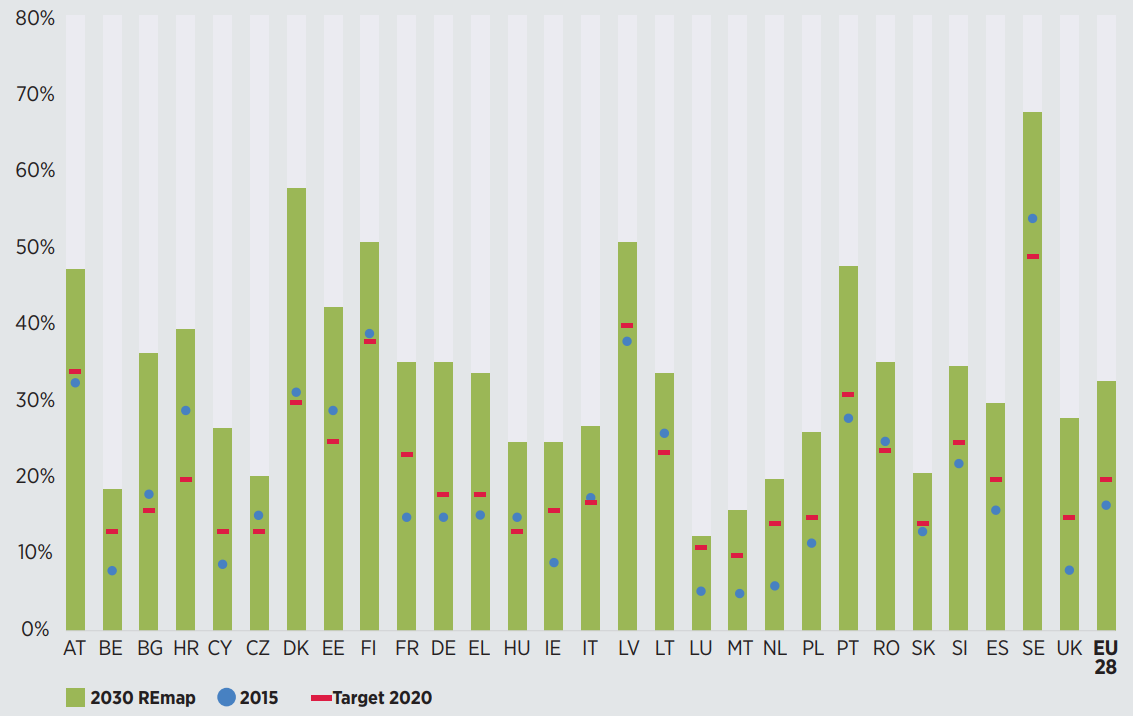
\includegraphics[scale=0.47]{EU2030.png}
	\caption{Renewable energy share in total energy consumption by EU for 2015, 2020 targets and 2030 potential according to REmap \cite{EuropeanCommission2018}}
	\label{EU2030}
\end{figure}

Renewable shares of REmap countries in 2010, 2030 reference case and 2030REmap and the world average is also shown in Figure \ref{2030map}. The only country whose renewable energy decreases in the 2030 is Nigeria. The reason is the main source of energy in Nigeria is biogas for the time being. However, the renewable share is expected to decrease dramatically as the industry switches to natural gas.
\begin{figure}[h!]
	\centering
	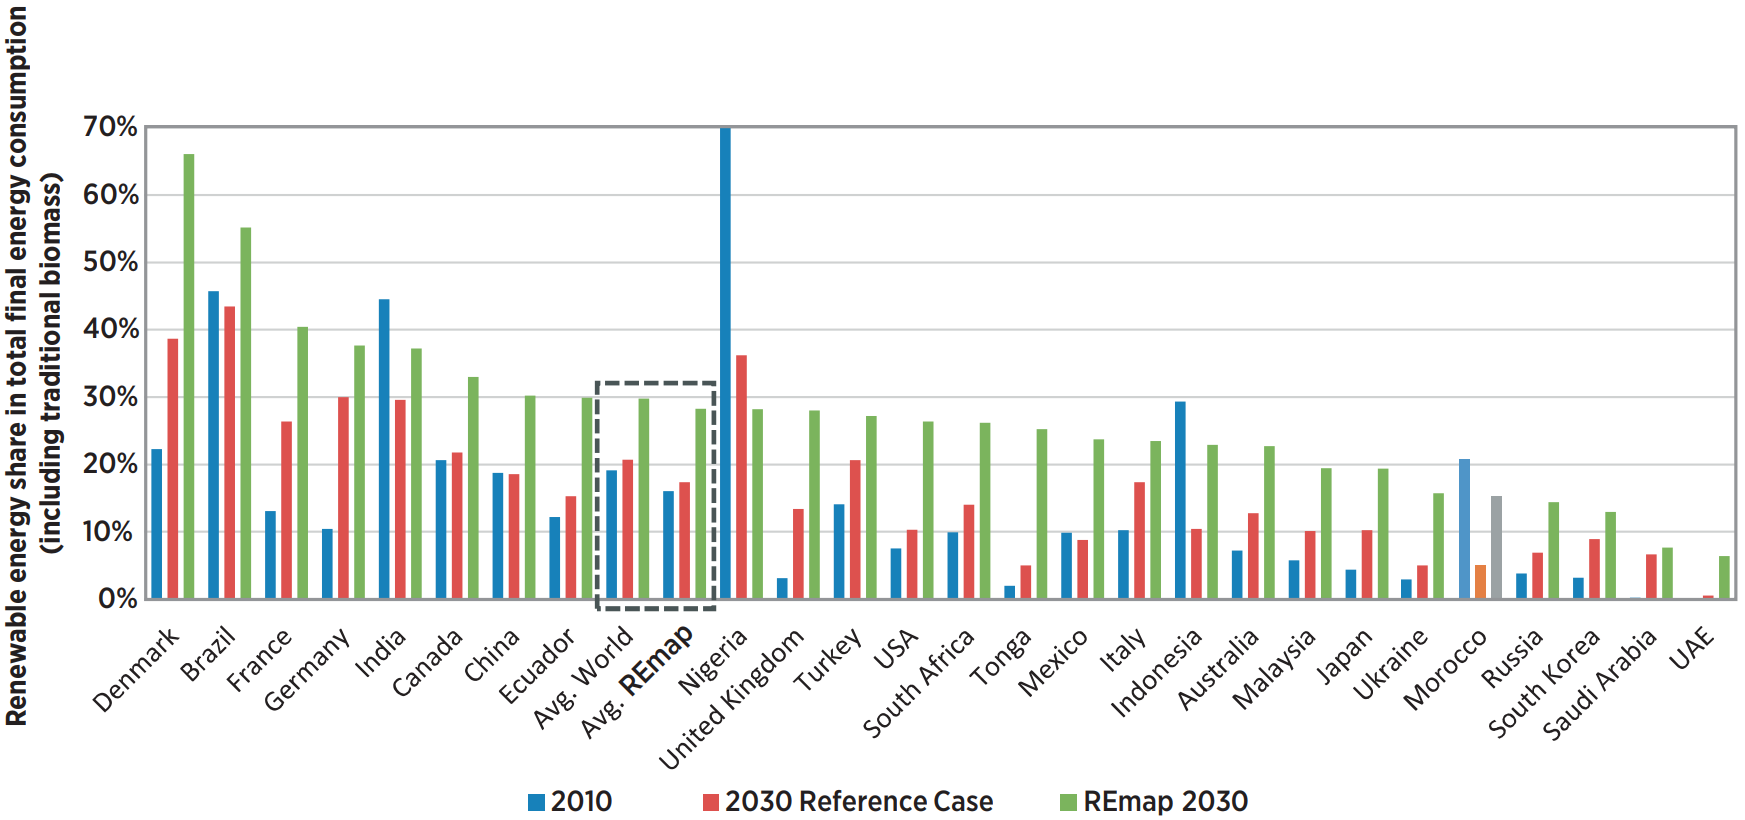
\includegraphics[scale=0.3]{2030map2.png}
	\caption{Renewable energy shares for 2010, 2030 Reference Case and 2030REmap \cite{IRENA2014}}
	\label{2030map}
\end{figure}

























